\chapter{Application mobile}

	\section{API REST}

		\subsection{Organisation des packages}

			%TODO Léa : Image et décrire le but des packages (src)

		\subsection{Parler configuration de l'application}

			\subsubsection{application.properties}

			L'API Rest possède un fichier application.properties qui permet de configurer certaines parties de l'application.

			\begin{figure}[H]
				\centering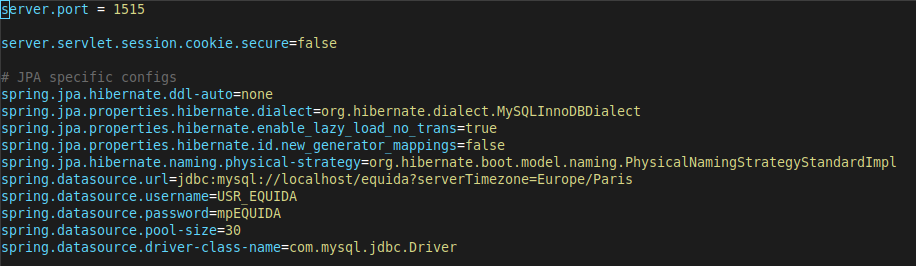
\includegraphics[width=0.85\textwidth, keepaspectratio]{res/application-properties.png}
				\caption{Configuration par application.properties}
			\end{figure}

			Dans ce fichier configure les informations relatives à l'application dans sa globalité, comme le port à utiliser, la configuration pour connexion avec la \bdd{} (nom utilisateur, mot de passe, ip, ...).

			\subsubsection{Configuration par le code}

			La configuration de Spring Security est directement faite dans le code source grace à l'utilisation de l'annotation "Configuration".

			\begin{figure}[H]
				\centering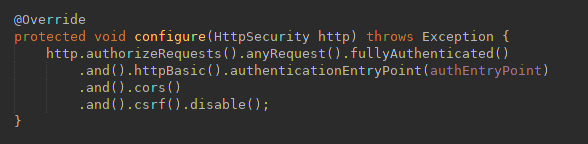
\includegraphics[width=0.75\textwidth, keepaspectratio]{res/config-httpsecurity.png}
				\caption{Configuration de Spring Security}
			\end{figure}

			Ici, on exige l'authentification sur toutes les requêtes faites à l'API. Celle ci doit être faite en utilisant Basic Authentification (voir \nameref{subsec:basic_auth}). On y active les CORS et on désactive le csrf.

			\begin{figure}[H]
				\centering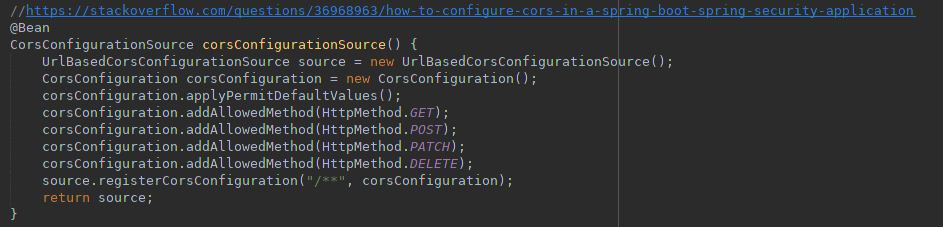
\includegraphics[width=0.75\textwidth, keepaspectratio]{res/config-cors.png}
				\caption{Configuration des requêtes CORS}
			\end{figure}

			Afin de permettre l'utilisation des requêtes DELETE et PATCH sur l'API, il a fallu changer la configuration des CORS. Le choix a été fait d'autoriser ces requêtes pour toutes les URL afin de simplifier la chose. Pour un code plus propre, il aurait fallu autoriser uniquement ce dont chaque URL utilisait.

			\begin{figure}[H]
				\centering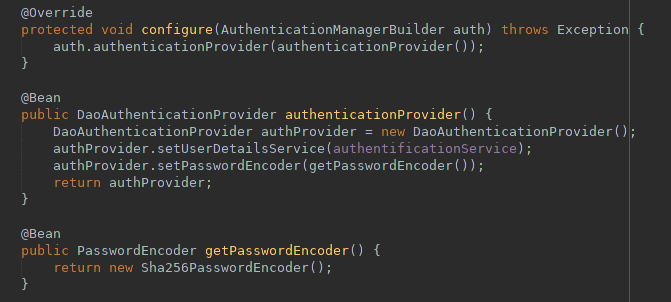
\includegraphics[width=0.75\textwidth, keepaspectratio]{res/config-authentification.png}
				\caption{Configuration de l'authentification}
			\end{figure}

			Enfin, comme pour WebApp, on définit le fonctionnement de l'authentification. Ainsi, vous pouvez retrouver les explications dans \nameref{par:authentification}.

		\subsection{Système d'authentification sur l'API}
			\label{subsec:basic_auth}

			L'api utilisant Basic Authentification il est nécessaire de fournir à Spring Security une implémentation de ce modèle. C'est le rôle d'AuthenticationEntryPointImpl dont voici le code :

			\begin{figure}[H]
				\centering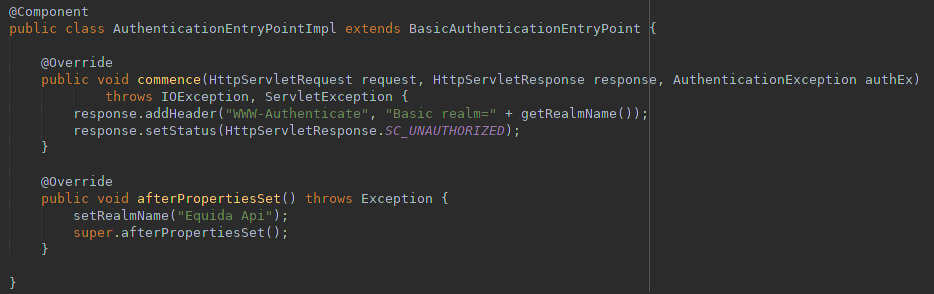
\includegraphics[width=0.75\textwidth, keepaspectratio]{res/AuthenticationEntryPointImpl.png}
				\caption{Code d'AuthenticationEntryPointImpl}
			\end{figure}

			Le code reste extrèmement simple ici car Spring Security nous offre une couche d'abstraction pour l'implémentation du modèle. Ainsi, le seul élément que l'on définit est le realm.

		\subsection{Exemple Route}

			%TODO Léa : Expliquer les méthodes de l'interface IRoute et donner un exemple de route.

		\subsection{Les Dto}

			\subsubsection{L'interface IDto}

				Afin d'alléger les requêtes SQL à la \bdd{} et la sortie en JSON des classes métiers, le choix à été fait d'utiliser les DTO. Aucun lien vers un autre objet n'est fait, seul son ID est laissé et il faudra ensuite utiliser l'URL adéquate afin de récupérer les informations si celles ci nous intéressent.

				Pour uniformiser nos Dto, une interface IDto a été faite.

				\begin{figure}[H]
					\centering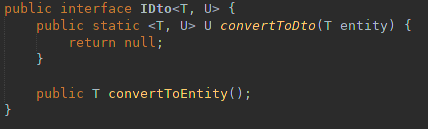
\includegraphics[width=0.75\textwidth, keepaspectratio]{res/idto.png}
					\caption{Code de l'interface IDto}
				\end{figure}

				Celle ci se base donc sur une généricité double, T étant notre classe métier provenant du package "com.equida.common.bdd.entity" et U étant la classe Dto correspondante. Cette interface définit 2 méthodes, "<T, U> U convertToDto(T entity)" permettant de convertir une instance de nos classe métier en un Dto et "T convertToEntity()" permettant de convertir notre Dto en une instance de nos classe métiers.

			\subsubsection{Exemple de Dto}

				%TODO Léa : Donner un exemple

		\subsection{Exemple Controller}

			%TODO Léa : Donner un exemple de controller

	\section{Ionic}

		\subsection{Organisation des packages}

			%TODO Léa : Image et décrire le but des packages (src)

		\subsection{Les pages}

			%TODO Léa : Parler de la nommenclature

			\subsubsection{Lister}

					%TODO Léa : Donner un exemple

			\subsubsection{Consulter}

					%TODO Léa : Donner un exemple

			\subsubsection{Ajouter}

					%TODO Léa : Donner un exemple

			\subsubsection{Modifier}

					%TODO Léa : Donner un exemple

		\subsection{Rest Api}

			Pour faciliter l'execution des différentes requêtes à l'API la classe "rest-api.service" a été conçue.

			\subsubsection{Authentification à l'Api}

				\begin{figure}[H]
					\centering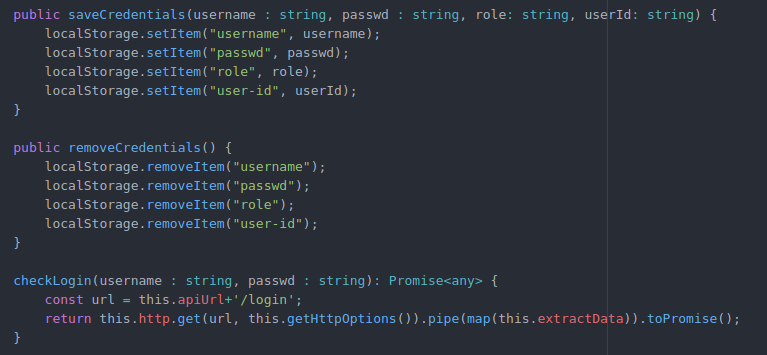
\includegraphics[width=0.75\textwidth, keepaspectratio]{res/ionic-rest-auth.png}
					\caption{Code de l'interface IDto}
				\end{figure}

				Ici, "saveCredentials" permet d'enregistrer les informations relatives à l'authentification du client dans le local storage. Il existe "removeCredentials" qui elle, à l'inverse de saveCredentials, supprime les informations relatives à l'utilisateur connecté. On a ainsi 2 méthodes qui permettent de gérer facilement la connexion et la déconnexion d'un utlisateur.

  				La méthode "checkLogin" permet de d'appeller "/api/login" et d'obtenir les informations relatives à l'utilisateur si les informations fournis sont correctes.

				\begin{figure}[H]
					\centering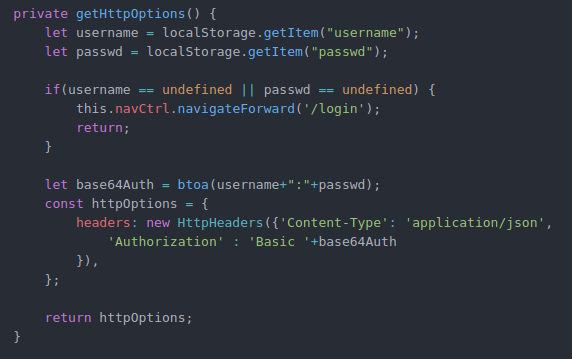
\includegraphics[width=0.75\textwidth, keepaspectratio]{res/ionic-rest-httpoptions.png}
					\caption{Code de l'interface IDto}
				\end{figure}

				Ces informations sont ensuite réutilisées pour permettre l'authentification à l'API. Pour cela la méthode "getHttpOptions" permet d'obtenir l'entête à founir à chaque appel à l'API. Dans le cas où le mot de passe ou le login est null, on redirige l'utilisateur vers la page de connexion.

			\subsubsection{Execution des différentes méthodes}

				Les appels à l'API utilisant les méthode HTTP GET, POST, PATCH et DELETE, une méthode existe, dans la classe "rest-api.service", pour chacune de ces méthodes HTTP. Voici un exemple avec la méthode HTTP GET.

				\begin{figure}[H]
					\centering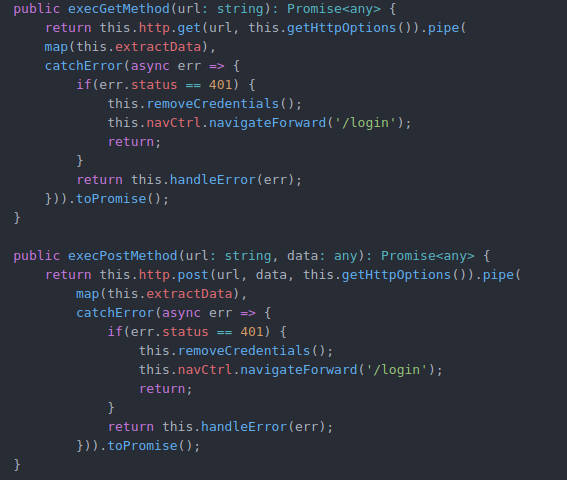
\includegraphics[width=0.75\textwidth, keepaspectratio]{res/ionic-rest-execmethod.png}
					\caption{Code de l'interface IDto}
				\end{figure}

				On effectue ici l'appel à l'url fournit en paramètre tout en récupérant les entêtes nécessaire pour l'authentification puis, selon que l'appel ai réussi ou non, on retourne le résultat ou on appel handleError afin de générer un message d'erreur ainsi qu'une exception. Il est important de vérifier si le code d'erreur est 401 car si c'est le cas, l'utilisateur est ou désactivé ou alors a son mot de passe de changé. Si tel est le cas, on le déconnexte et on le redirige vers la page de connexion.

				Les autres méthodes ne change pas tellement si ce n'est que pour POST et PATCH on fournis en plus un objet "data" qui correspond aux informations à fournir à l'API mais aussi que le nom des méthodes appellées sur l'objet http change.

				\begin{figure}[H]
					\centering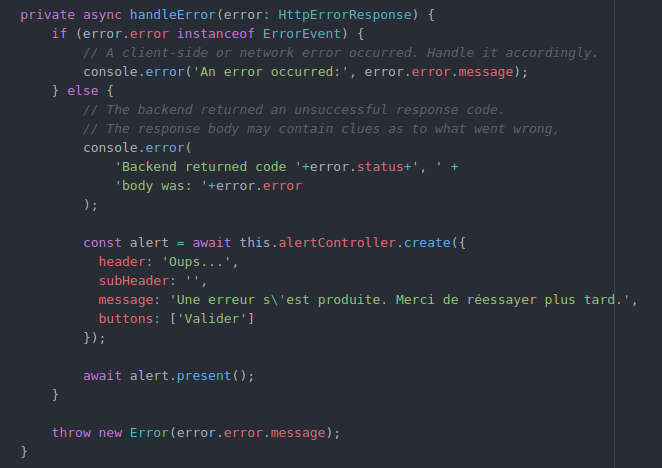
\includegraphics[width=0.75\textwidth, keepaspectratio]{res/ionic-rest-error.png}
					\caption{Code de l'interface IDto}
				\end{figure}

				La méthode "handleError" affiche les informations relatives à l'erreur dans la console du navigateur et se charge également d'afficher une boite de dialogue expliquant qu'une erreur est surveneue. Dans le cadre du développement, cela permet également de rappeller que plus d'informations sont disponibles dans la console.

			\subsubsection{Exemples}

			Ainsi, l'appel aux différents endpoints de l'API tient en quelques lignes et se retrouve extrèmement simpifié comme on peut le voir sur les méthodes suivantes :

				\begin{figure}[H]
					\centering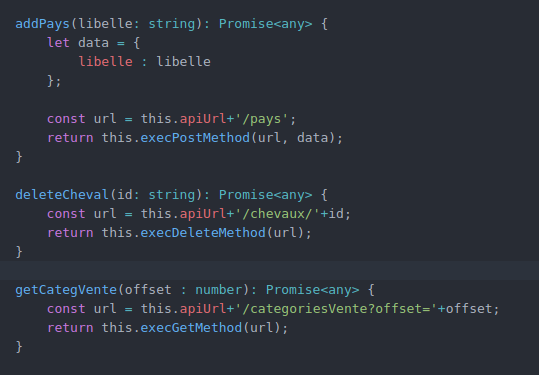
\includegraphics[width=0.75\textwidth, keepaspectratio]{res/ionic-rest-add-delete-get.png}
					\caption{Code de l'interface IDto}
				\end{figure}

			Le fait de retourner une instance de Promise permet d'utiliser "await" sur la méthode et donc d'attendre la réponse de l'API avant de continuer l'execution du code.

		\subsection{Problèmes connus}

			%TODO Léa : Parler refresh si ajout ou modif

			Actuellement, en cas d'erreur sur les formulaires, une boite de dialogue avec un message expliquant qu' "une erreur est survenue" s'affiche. A terme il faudrait afficher un message sur l'écran expliquant le champs sur lequel l'erreur est survenue ainsi que la raison de celle ci. Cela est actuellement impossible à faire car il faut restructurer la façon donc rest-api.service fonctionne afin d'y permettre, d'une part, une meilleure gestion des erreurs, d'autre partle fait de ne pas afficher la boite de dialogue systématiquement dans le cas où l'API retourne un code d'erreur.
